\documentclass[12pt]{article}
\usepackage[utf8]{inputenc}
\usepackage[spanish]{babel}
\usepackage{amsmath, amssymb}
\usepackage{graphicx}
\usepackage{float}
\usepackage{hyperref}
\usepackage{geometry}
\geometry{margin=2.5cm}

\title{Agente Inteligente para el Juego de Hex}
\author{Javier A. González Díaz \\ Facultad de Matemática y Computación}
\date{\today}

\begin{document}

\maketitle


\begin{figure}[H]
    \centering
    
\includegraphics[width=0.15\textwidth]{img/matcom.jpg}
    \label{fig:matcom}
\end{figure}

\section*{Resumen}
Este informe describe el diseño e implementación de un agente inteligente para el juego de Hex, desarrollado como parte de la asignatura de Inteligencia Artificial. El agente utiliza una combinación de algoritmos de búsqueda como Minimax con poda alfa-beta, el algoritmo A* para estimar distancias mínimas, y una heurística basada en conexiones virtuales (puentes seguros)
que asegura un juego estratégico y equilibrado.Además se utilizan técnicas de filtrado , conteo y ordenación para lograr mejores tiempos de ejecución.

\section{Introducción}
El juego de Hex es un juego de estrategia para dos jugadores, cuyo objetivo es conectar lados opuestos del tablero con fichas propias. Debido a su naturaleza determinista y su gran espacio de estados, es un candidato ideal para aplicar técnicas de Inteligencia Artificial y demostrar control de tiempo en tomas de decisiones sin sacrificar efectividad.

\begin{figure}[H]
    \centering
    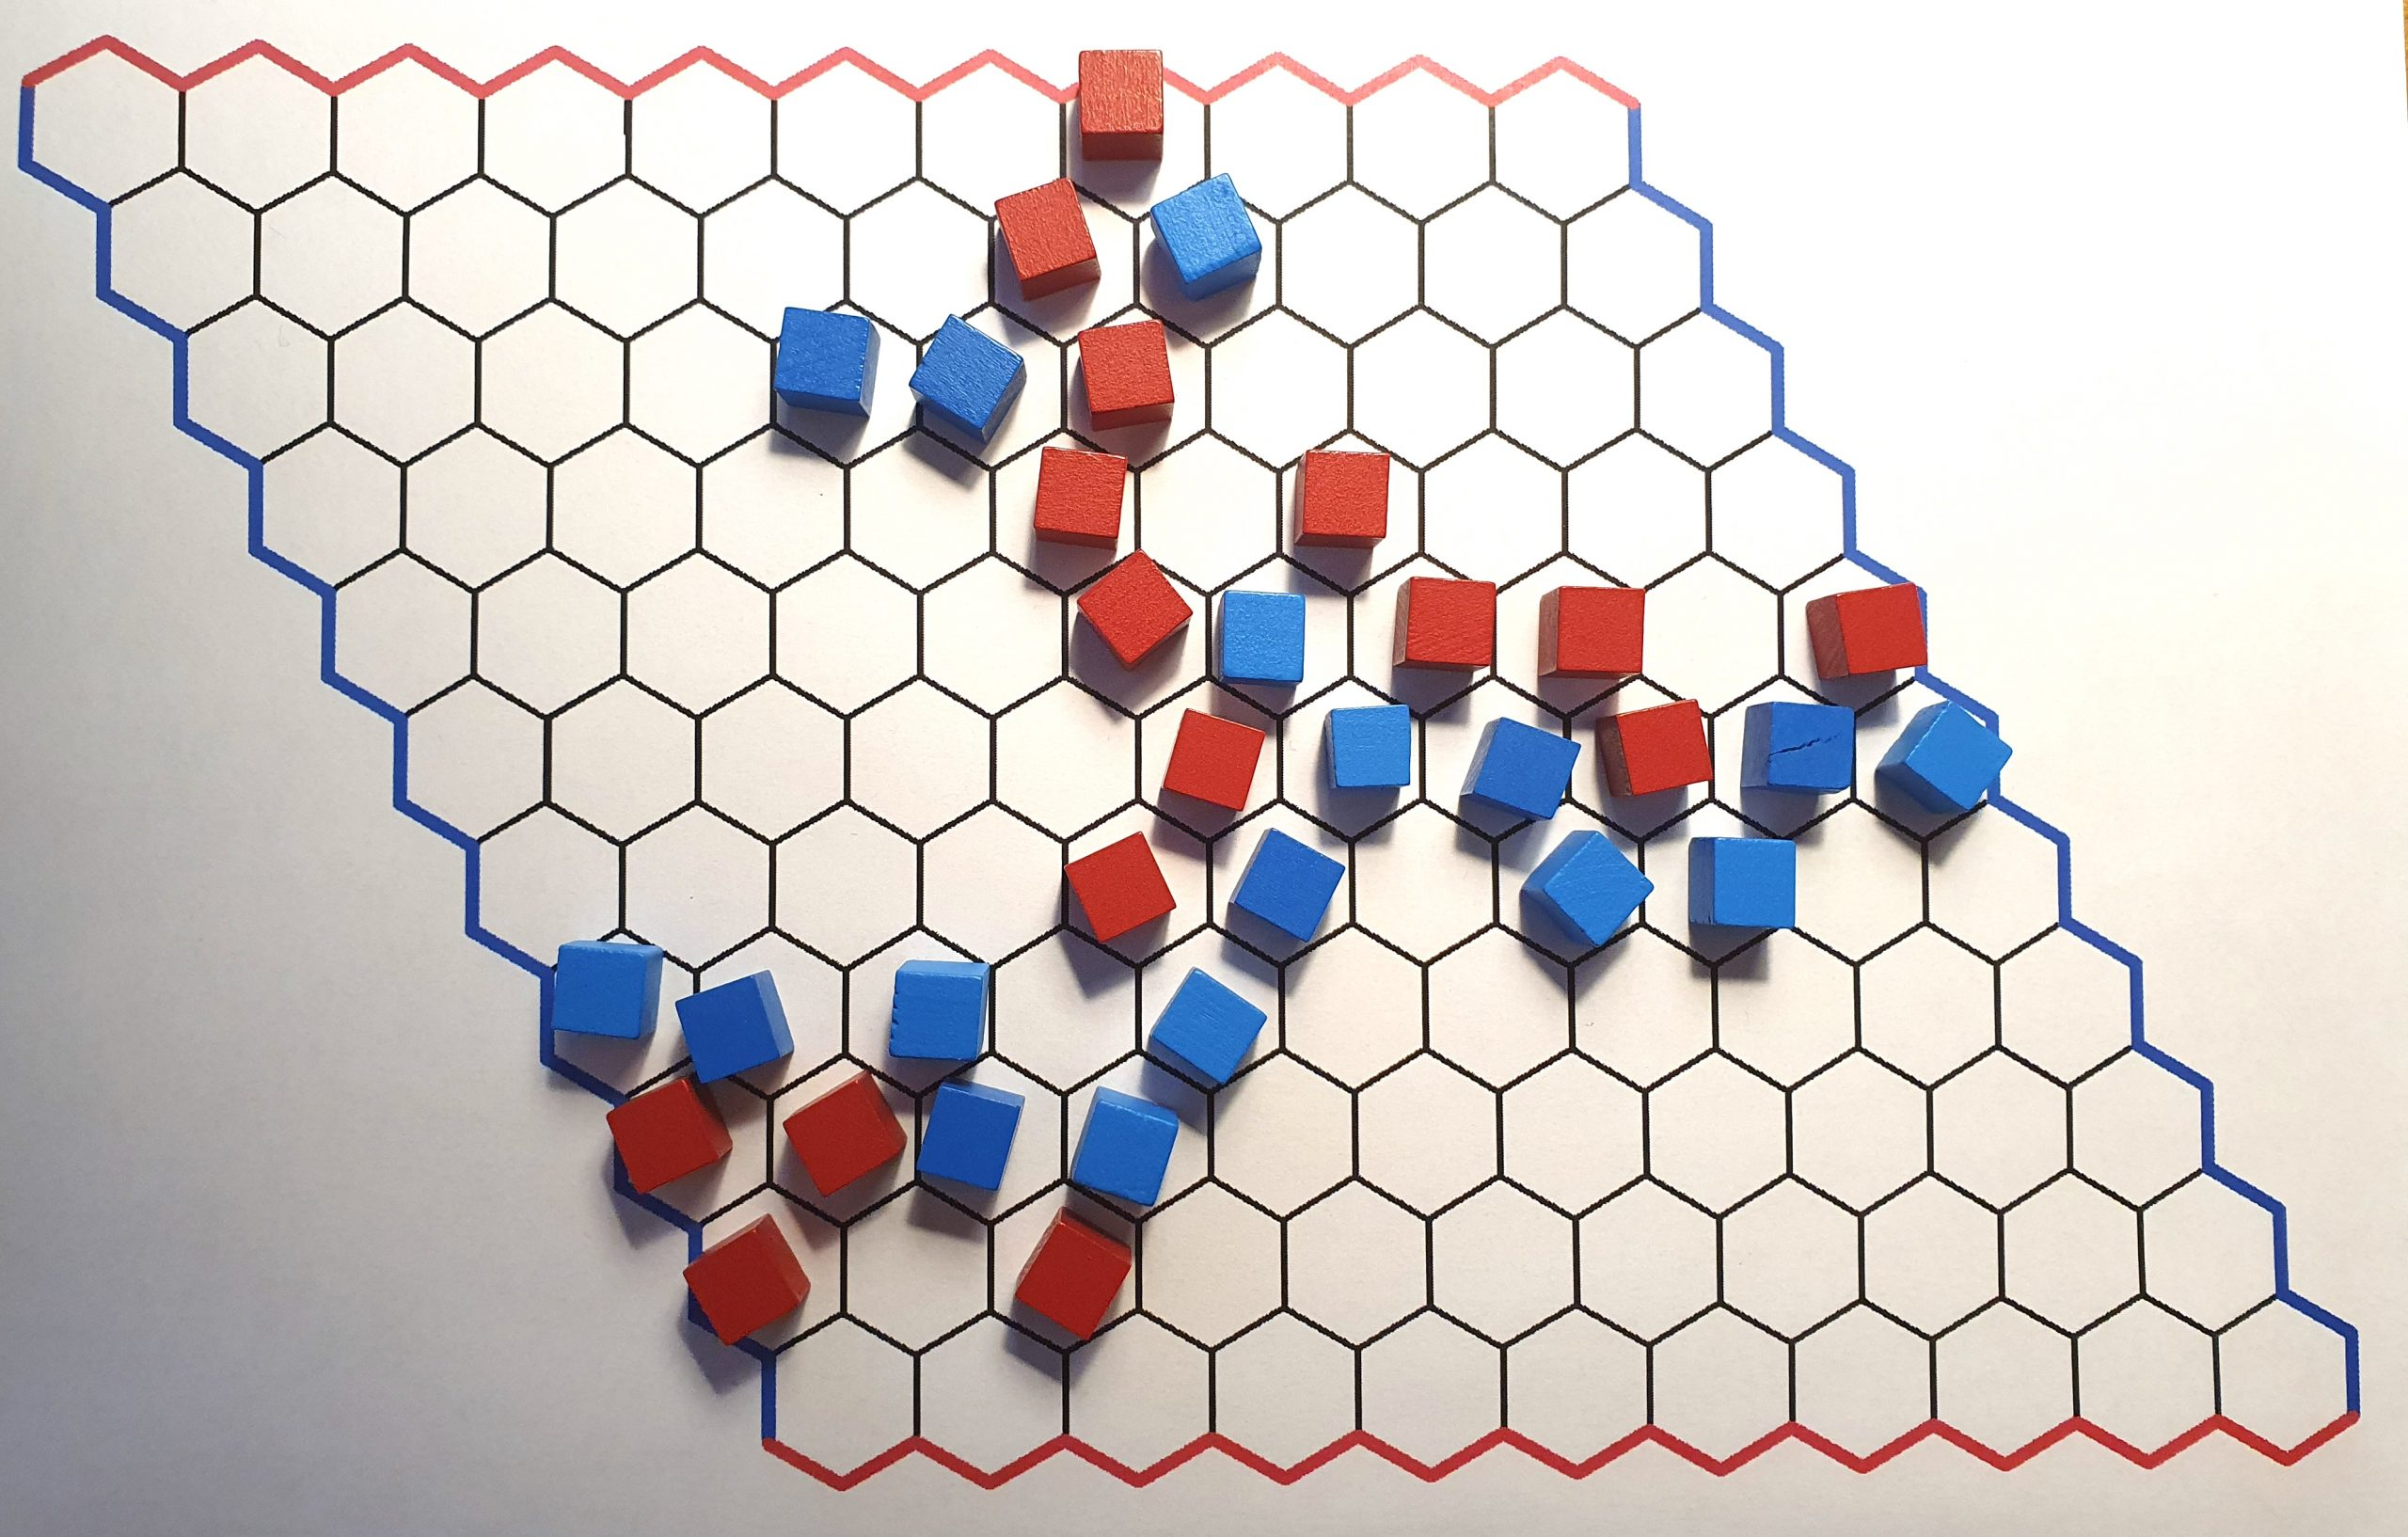
\includegraphics[width=0.3\textwidth]{img/hex_board.jpg}
    \caption{Tablero de HEX.}
    \label{fig:hex_board}
\end{figure}

\section{Algoritmo Minimax con Poda Alfa-Beta}
El núcleo de decisión del agente es el algoritmo Minimax, que explora los posibles movimientos futuros para elegir el más prometedor. Para mejorar la eficiencia, se implementó poda alfa-beta, lo cual reduce el número de nodos evaluados sin afectar el resultado.

\[
\text{Minimax}(estado, profundidad, \text{jugador}) = 
\begin{cases}
\text{valor heurístico} & \text{si profundidad = 0 o estado terminal} \\
\max(\text{Minimax}(hijo)) & \text{si es turno del jugador} \\
\min(\text{Minimax}(hijo)) & \text{si es turno del oponente}
\end{cases}
\]

\section{Función de Evaluación}
La función de evaluación combina múltiples factores para estimar la conveniencia de una posición:

\[
f(s) = w_1 \cdot f_1 + w_2 \cdot f_2 + w_3 \cdot f_3
\]

donde:
\begin{itemize}
  \item \( f_1 \): diferencia entre el costo mínimo de camino del oponente y del jugador (calculado con A*),
  \item \( f_2 \): diferencia de conexiones virtuales seguras (puentes seguros),
  \item \( f_3 \): diferencia de cantidad de fichas colocadas.
\end{itemize}

Con los pesos:
\[
w_1 = 0.8,\quad w_2 = 0.3,\quad w_3 = 0.2
\]

\section{A* para Costo del Camino Mínimo}

El algoritmo A* se utiliza para estimar el costo mínimo que un jugador necesita para conectar sus lados del tablero. En Hex, el tablero puede modelarse como un grafo donde cada celda es un nodo conectado a sus seis vecinos inmediatos. Esta representación permite aplicar técnicas clásicas de búsqueda en grafos.

\subsection{Cálculo del Camino Mínimo}

Para cada jugador, se definen las -celdas fuente- como aquellas situadas en el borde inicial (superior o izquierdo, según el jugador), y el objetivo es alcanzar el borde opuesto (inferior o derecho).

El algoritmo A* combina el costo real acumulado \( g(n) \) desde el inicio hasta el nodo actual, con una heurística \( h(n) \) que estima la distancia restante hasta el objetivo. En este caso:

\[
h(r, c) = 
\begin{cases}
n - 1 - c, & \text{si el jugador conecta de izquierda a derecha} \\
n - 1 - r, & \text{si conecta de arriba a abajo}
\end{cases}
\]

Esta heurística representa una estimación optimista de la distancia, que asume que el jugador puede avanzar sin obstáculos hasta su meta. Esto garantiza que A* sea **admisible**, es decir, que nunca sobreestima el costo real.

Cada celda se evalúa con el siguiente criterio de costo:

\begin{itemize}
  \item Si está ocupada por el jugador: \( \text{costo} = 0 \)
  \item Si está vacía: \( \text{costo} = 1 \)
  \item Si está ocupada por el oponente: \( \text{costo} = \infty \)
\end{itemize}

Este enfoque prioriza caminos ya parcialmente controlados por el jugador , interrumpe caminos construidos por el oponente y penaliza severamente las obstrucciones de este.

\subsection{Utilidad en la Evaluación}

El valor devuelto por A* representa la cantidad mínima de movimientos necesarios (en el mejor de los casos) para que el jugador conecte sus lados. Se compara con el costo estimado del oponente, y esta diferencia se utiliza como componente principal en la función de evaluación:

\[
f_1 = \text{costo}_{\text{oponente}} - \text{costo}_{\text{jugador}}
\]

Cuanto menor sea el costo del jugador respecto al del oponente, más prometedora es la posición para el agente.

\section{Puentes Seguros (Safe Bridges)}
Los \textit{safe bridges} son patrones de conexión virtual que, aunque no estén ocupados, representan enlaces estratégicos que solo el jugador puede completar en futuras jugadas. Se utilizan para detectar ventaja posicional y se cuentan dinámicamente durante la evaluación de los nodos.

\begin{figure}[H]
    \centering
    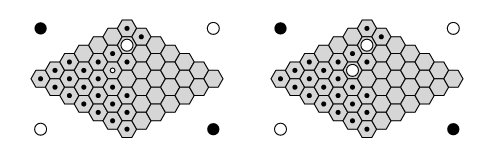
\includegraphics[width=0.4\textwidth]{img/safe-bridge.png}
    \caption{Ejemplo de puente seguro entre las dos fichas blancas.}
    \label{fig:safe_bridge}
\end{figure}

\paragraph{}
El uso de \textit{safe bridges} o conexiones virtuales es una técnica reconocida en entornos profesionales de Hex. Estos patrones permiten prever futuras conexiones seguras que el oponente no puede bloquear completamente en un solo turno. Esta capacidad de anticipación estratégica distingue a jugadores avanzados, y su inclusión en un agente automático refuerza la calidad de su juego posicional.


\section{Filtrado y Selección Eficiente de Jugadas}

El agente genera un conjunto reducido de movimientos relevantes en cada turno, evitando recorrer todo el tablero. Esto se logra mediante filtros centrados en las zonas activas del juego y en estructuras estratégicas como los puentes.Esta estrategia permite evitar considerar movimientos irrelevantes o lejanos al contexto estratégico actual, mejorando así el rendimiento en cada iteración de \texttt{minimax}.

La función \texttt{get\_relevant\_moves} combina:
\begin{itemize}
  \item Vecinos vacíos de las fichas del jugador (para expandir conexiones).
  \item Vecinos vacíos de las fichas del oponente (para bloquear).
  \item Celdas que podrían formar \textit{puentes seguros} con fichas propias.
\end{itemize}

Los puentes seguros se identifican cuando dos fichas no adyacentes comparten exactamente dos vecinos vacíos, lo cual permite prever conexiones virtuales resistentes a bloqueos. Las funciones \texttt{get\_potential\_bridges} y \texttt{bridge\_neighbors} encapsulan esta lógica.

Para la apertura, se prioriza el centro del tablero y, si está ocupado, se elige un vecino aleatorio.

Gracias a esta estrategia de filtrado:
\begin{itemize}
  \item Se reduce drásticamente el espacio de búsqueda.
  \item Se mantiene un enfoque táctico, tanto ofensivo como defensivo.
  \item Se mejora la eficiencia del algoritmo \texttt{minimax}, permitiendo mayor profundidad sin penalizar el rendimiento.
\end{itemize}

\end{document}